\chapter{Introdução}\label{cap:introducao}

O suprimento contínuo de energia elétrica condiciona a operação de sistemas de produção industrial, centros de saúde e redes de comunicação. Nesse ecossistema de infraestrutura, os transformadores de potência atuam como elementos centrais na conversão de níveis de tensão e corrente nas etapas de geração, transmissão e distribuição. A operação em regime ininterrupto sob carregamento dinâmico e estresses ambientais impõe desgaste contínuo aos materiais internos, podendo culminar em falhas catastróficas que acarretam interrupções de fornecimento e elevados custos de recomposição patrimonial \cite{tightiz2020}. Por esse motivo, o monitoramento contínuo da integridade operacional desses equipamentos constitui prática indispensável para a engenharia de manutenção.

A degradação dos componentes internos decorre primariamente de solicitações térmicas e dielétricas aplicadas sobre o sistema de isolamento composto por óleo mineral e papel celulósico. As reações de clivagem molecular provocadas por aquecimentos localizados e descargas elétricas induzem a liberação de espécies gasosas que se dissolvem no fluido dielétrico, incluindo hidrogênio ($\text{H}_2$), metano ($\text{CH}_4$), etano ($\text{C}_2\text{H}_6$), etileno ($\text{C}_2\text{H}_4$) e acetileno ($\text{C}_2\text{H}_2$), acompanhados por monóxido de carbono ($\text{CO}$) proveniente da isolação sólida. A mensuração periódica dessas concentrações por cromatografia gasosa, denominada Análise de Gases Dissolvidos (\textit{Dissolved Gas Analysis}, DGA), constitui a principal metodologia de diagnóstico incipiente de falhas \cite{ali2023}.

A cadeia causal que vincula a operação do equipamento ao diagnóstico físico-químico está ilustrada na Figura~\ref{fig:cadeia_causal}. As solicitações de campo degradam o isolamento, gerando subprodutos gasosos cuja assinatura estequiométrica reflete o regime de temperatura e a intensidade energética da falha. Tradicionalmente, esses dados são interpretados por métodos baseados em regras geométricas ou razões estáticas pré-fixadas, os quais atuam de forma reativa após a consolidação do defeito. Em contraste, abordagens orientadas a dados buscam modelar a dinâmica de evolução gasosa e otimizar a identificação de anomalias por meio de inteligência computacional.

\begin{figure}[htbp]
\centering
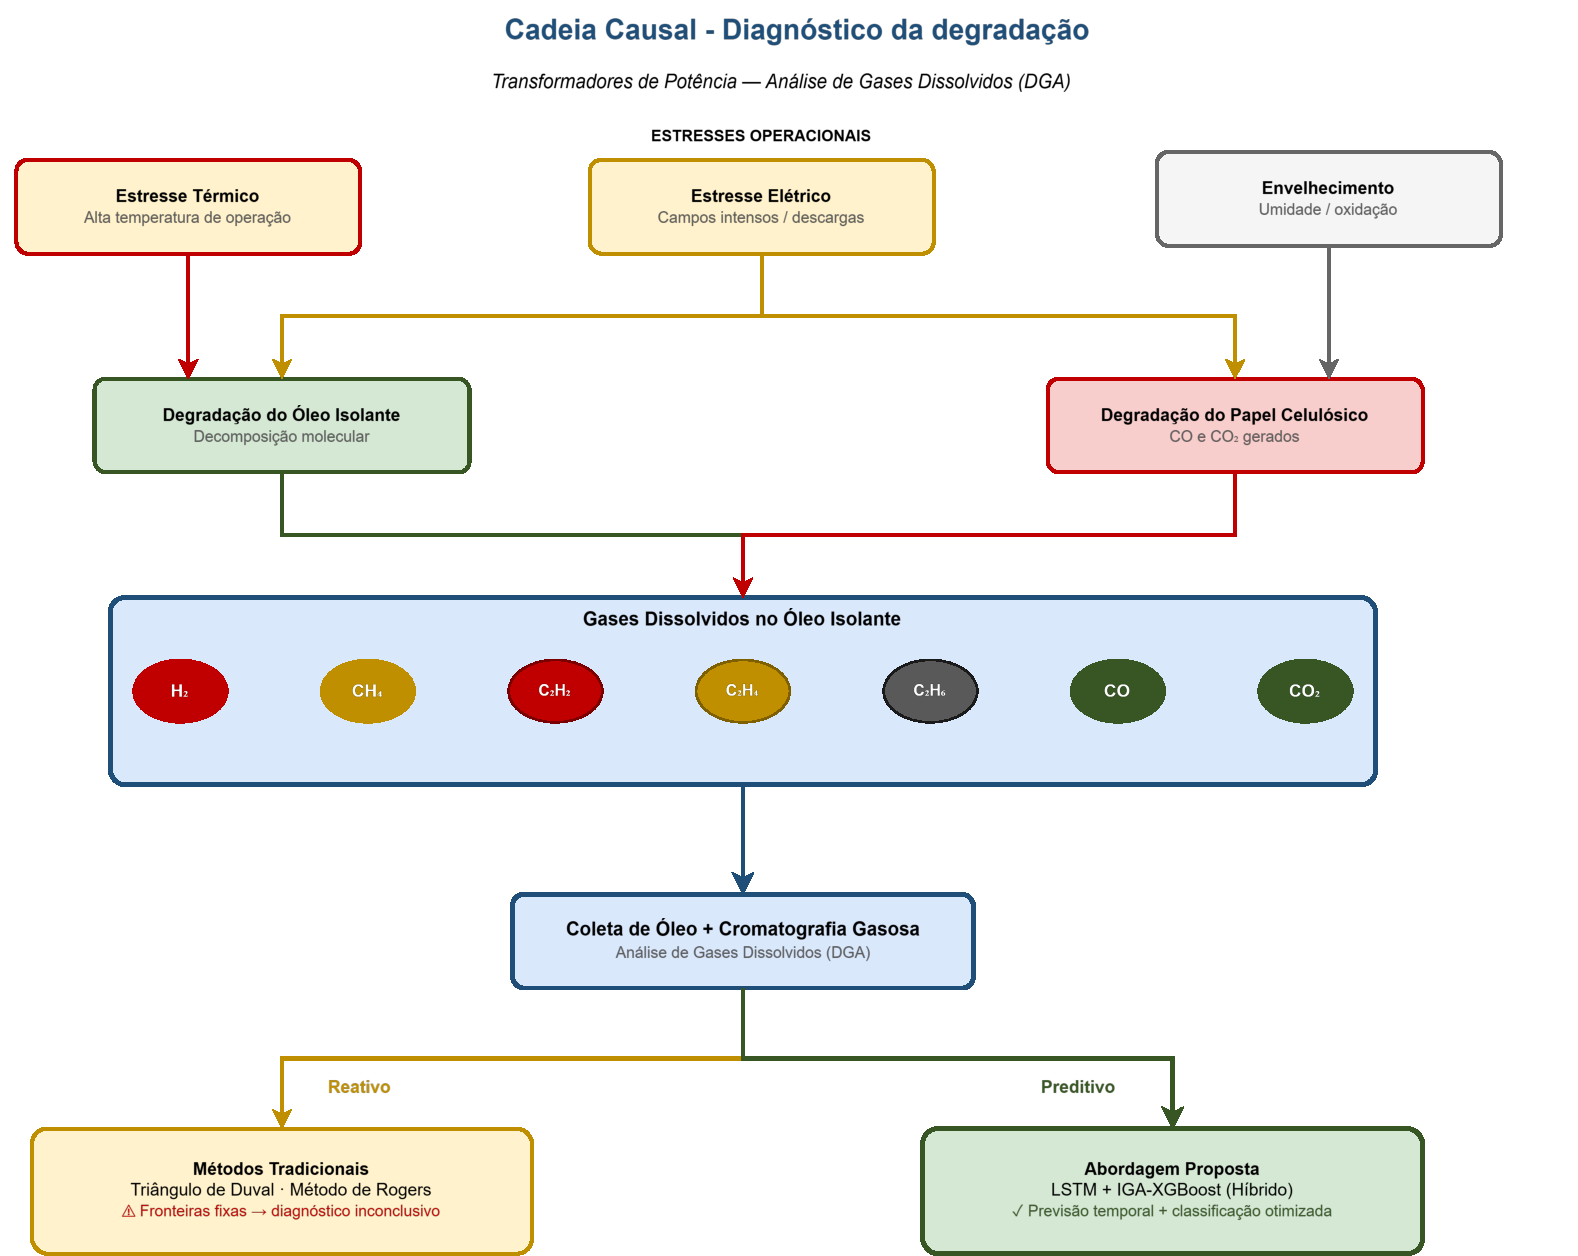
\includegraphics[width=\textwidth]{figuras/Cadeia_causal.pdf}
\caption{Cadeia causal da degradação de transformadores de potência e DGA, confrontando a abordagem normativa reativa com a modelagem preditiva orientada a dados.}
\label{fig:cadeia_causal}
\fonte{Elaborado pelo autor.}
\end{figure}

A aplicação prática de técnicas de aprendizado de máquina no domínio de DGA enfrenta, contudo, uma restrição imposta pela natureza dos dados abertos disponíveis. Constata-se na literatura uma assimetria estrutural entre bases temporais contínuas, que registram leituras periódicas de sensores online restritas a subconjuntos de gases, e bases estáticas consolidadas, que cobrem os cinco gases normativos e a taxonomia completa de falhas, porém sem rastreamento longitudinal. Diante dessa condição de contorno, a presente pesquisa investiga a integração entre projeções temporais e algoritmos de classificação estática a partir de um desenho metodológico estruturado em dois eixos experimentais complementares, incorporando procedimentos rigorosos de teste de hipótese e interpretabilidade físico-química pós-hoc.

\section{Tema}\label{sec:tema}

O tema deste trabalho consiste na investigação empírica de arquiteturas híbridas baseadas em redes neurais recorrentes LSTM e algoritmos XGBoost otimizados por algoritmos genéticos, com foco na avaliação ablativa de projeções temporais, busca por parcimônia dimensional e validação físico-química de falhas em transformadores de potência por Análise de Gases Dissolvidos.

\section{Justificativa}\label{sec:justificativa}

Os métodos normativos tradicionais de diagnóstico em DGA, como o Triângulo 1 de Duval e o Método das Razões da IEC 60599, operam a partir de fronteiras poligonais rígidas e tabelas discretas de corte. Embora consolidados na prática industrial, esses métodos apresentam limitações estruturais documentadas, destacando-se a ausência de definição de estado de operação normal e a elevada taxa de diagnósticos indeterminados em amostras com sinais de degradação mista \cite{alsakini2025}. Tais restrições motivaram a adoção crescente de algoritmos de aprendizado supervisionado, como o XGBoost, capazes de mapear fronteiras de decisão não lineares a partir de medições cromatográficas \cite{wu2021}.

Não obstante os avanços reportados na literatura, a maioria das soluções propostas opera estritamente sobre registros pontuais estáticos, ignorando a dinâmica temporal da gaseificação, ou formula modelos híbridos sob a premissa teórica de que projeções temporais geradas por redes recorrentes obrigatoriamente elevam o desempenho discriminativo de classificadores estáticos \cite{wang2023}. Essa hipótese, contudo, raramente é submetida a protocolos formais de ablação estatística com intervalos de confiança e testes pareados. Adicionalmente, modelos complexos baseados em ensembles de árvores são frequentemente tratados como sistemas opacos, sem auditoria formal da concordância entre as fronteiras estocásticas aprendidas e os princípios termodinâmicos postulados nas normas técnicas da engenharia de alta tensão.

Torna-se justificável, portanto, conduzir uma investigação científica rigorosa que audite a real contribuição informacional de projeções temporais de curto e médio prazo, quantifique o ganho de parcimônia propiciado por algoritmos evolutivos na seleção de variáveis e estabeleça uma ponte analítica entre modelos de aprendizado de máquina e as normas clássicas de DGA por meio de métodos axiomáticos de interpretabilidade.

\section{Objetivos}\label{sec:objetivos}

O objetivo geral deste trabalho consiste em desenvolver, auditar e avaliar experimentalmente uma abordagem computacional para o diagnóstico de falhas em transformadores de potência a partir de dados de DGA, investigando o valor incremental de projeções temporais via redes LSTM, a parcimônia dimensional proporcionada pelo Algoritmo Genético Melhorado acoplado ao XGBoost e a conformidade físico-química das decisões frente às normas internacionais por meio de técnicas de interpretabilidade.

Para concretizar a proposta, definem-se os seguintes objetivos específicos.

O primeiro objetivo específico reside em auditar e preparar bases de dados reais de DGA, eliminando duplicidades amostrais que induzam viés estatístico e estruturando a experimentação em dois eixos analíticos fundamentados na disponibilidade de variáveis físico-químicas.

O segundo objetivo específico visa implementar um módulo de previsão temporal baseado em redes neurais recorrentes LSTM empilhadas para gerar estimativas pontuais de concentrações gasosas em múltiplos horizontes operacionais futuros.

O terceiro objetivo específico consiste em submeter a integração entre as projeções temporais da LSTM e o classificador XGBoost a um protocolo formal de ablação pareada por reamostragem estatística, quantificando com rigor inferencial o ganho informacional efetivo da hipótese temporal.

O quarto objetivo específico consiste em avaliar a capacidade do Algoritmo Genético Melhorado (IGA) em promover redução de dimensionalidade e seleção parcimoniosa de atributos, confrontando seu desempenho contra modelos padrão e limites teóricos de informação no diagnóstico de falhas.

O quinto objetivo específico reside em auditar a coerência físico-química dos padrões aprendidos pelo modelo supervisionado em relação aos limiares analíticos do Triângulo 1 de Duval e da norma IEC 60599, aplicando a formulação de valores de Shapley e o algoritmo TreeSHAP.

\section{Organização do Texto}\label{organizacao}

O trabalho está estruturado em cinco capítulos encadeados logicamente.

O Capítulo~\ref{Fundamentacao} apresenta a fundamentação teórica, cobrindo os transformadores de potência, os mecanismos físico-químicos de degradação do sistema de isolamento, os métodos normativos clássicos de DGA, os fundamentos matemáticos dos algoritmos de aprendizado de máquina e otimização evolutiva, a teoria axiomática dos valores de Shapley via TreeSHAP e a revisão crítica dos trabalhos relacionados.

O Capítulo~\ref{cap:metodologia} descreve os procedimentos metodológicos adotados, detalhando a divisão da pesquisa nos eixos Track A e Track B, os protocolos de auditoria e saneamento de dados, a engenharia de atributos, a parametrização dos modelos LSTM e IGA-XGBoost, os testes de significância estatística baseados em bootstrap pareado e validação cruzada repetida, e o protocolo de interpretabilidade pós-hoc.

O Capítulo~\ref{cap:resultados} expõe os resultados experimentais e as discussões técnicas correspondentes, abordando a capacidade preditiva da rede recorrente, o teste formal de ablação da hipótese temporal, a avaliação multiclasse de integridade operacional frente ao teto informacional da base de dados, a auditoria de concordância com os métodos tradicionais e a validação físico-química das fronteiras estocásticas por valores de Shapley.

O Capítulo~\ref{cap:conclusao} (Conclusão) sintetiza as contribuições científicas e práticas da pesquisa, apresenta a discussão técnica sobre os resultados experimentais negativos, reconhece as limitações decorrentes dos conjuntos de dados industriais disponíveis e delineia direcionamentos prioritários para trabalhos futuros.